\documentclass[a4paper,9pt]{beamer}

\setbeamercovered{transparent}
%\usepackage{ifthen}
\usepackage{caption}

\captionsetup{font=scriptsize,labelfont=scriptsize}

\setbeamertemplate{theorem begin}{{
\inserttheoremheadfont
\inserttheoremname
\inserttheoremnumber
\ifx \inserttheoremaddition \empty \else\ (\inserttheoremaddition)\fi%
\inserttheorempunctuation
\hspace{0.1cm}
}}
\setbeamertemplate{theorem end}{}

\newtheoremstyle{mytheoremstyle} % name
        {\topsep}                    % Space above
        {\topsep}                    % Space below
        {\itshape\fontfamily{ptm}\selectfont}                   % Body font
        {}                           % Indent amount
        {\fontfamily{ptm}\selectfont\scshape\color{blue}}                   % Theorem head font
        {:}                          % Punctuation after theorem head
        {.5em}                       % Space after theorem head
        {}  % Theorem head spec (can be left empty, meaning ‘normal’)
\theoremstyle{mytheoremstyle}


\newtheorem{hypothesis}{Hypothesis}
\newtheorem*{unnumberedhypothesis}{Hypothesis}
\newtheorem*{unnumberednullhypothesis}{Null Hypothesis}
\newtheorem{notion}{Notion}

%\usepackage{polski}
\usepackage[cp1250]{inputenc}
\usepackage{tcolorbox}
\usepackage{tikz}


\usetheme{Warsaw}
\setbeamercovered{transparent}


%\logo{\includegraphics[width=.1\textwidth]{res/logo_uam}}
\begin{document}

\title[Modeling of Polish Intonation for SPSS]{Modeling of Polish Intonation for Statistical-Parametric Speech Synthesis}
\author[Tomasz Kuczmarski]{Tomasz Kuczmarski\\
\vspace{0.5cm}
\small{Prof. zw. Dr hab. In\.z. Gra\.zyna Demenko}\\
\textit{\tiny{Supervisor}}}
\institute{\protect{\small{Adam Mickiewicz University}}\\
\includegraphics[width=.1\textwidth]{res/logo_uam}\\
\tiny{Faculty of Modern Languages and Literature}\\
\tiny{Institute of Ethnolinguistics}\\
}

% WYWALIĆ
\date{\tiny{May 18, 2022}}

%
\begin{frame}
\titlepage
\end{frame}




\begin{frame}
\frametitle{Intonation}
\framesubtitle{Definition}
\vspace{2cm}
\textit<1-2>{``The tonal structure of speech expressed by the melody produced by our larynx. It has a phonetic aspect, the fundamental frequency ($F0$), and a grammatical (phonological) aspect.''} (F\'ery 2016)
\begin{columns}
\column{0.5\textwidth}
\column{0.5\textwidth}
\vspace{0.5cm}
\invisible<1>{\begin{alertblock}{}
All definitions of intonation "are epistemological
definitions,i.e., not a priori programmatic definitions, but a posteriori statements of a practice and methodology." (Rossi 2000)
\end{alertblock}}
\end{columns}
\end{frame}

\section{Motivation}

\begin{frame}
\frametitle{Motivation}
\begin{columns}
\column{0.4\textwidth}
\begin{center}
\includegraphics[width=\textwidth]{res/mapping_highlight.png}
\end{center}
\column{0.6\textwidth}
\begin{exampleblock}{Motivation}
\begin{itemize}
\item[\checkmark] Epistemological definition of intonation.
\item[\checkmark] Dualistic gap between phonology and phonetics.
\item[\checkmark] Unification within a broader metatheory.
\item[\checkmark] Unknown nature of the mappings between mental categories and continuous contours of $F0$.
\item[\checkmark] Explore how linguistic features of an utterance influence its $F0$ contours.
\item[\checkmark] Need for a physicalist (neurobiological) model.
\item[\checkmark] Modern statstical-parametric speech synthesis provides a framework for experimentation and evaluation of such models.
\end{itemize}
\end{exampleblock}
\end{columns}
\end{frame}



\section{Objectives}
\subsection{Objectives}
\begin{frame}
\frametitle{Objectives}
\begin{enumerate}
\item<1-2> Build a robust biologically-inspired neural model of the probabilistic mapping between discrete low-level linguistic features of an utterance and its intonation contours ($F0$ values).
\item<2> Build a state-of-the-art neural source-filter resynthesis framework for Polish read speech.
\item<2> Deploy the intonation model within the resynthesis framework and measure the perceived naturalness of the output intonation contours, and to
\item<2> operationalize the results of these measurements as an indicator of the model's robustness.
\item<2> Develop a method to explain the relevance of the individual input linguistic features for the produced intonation contour.
\item<1-2> Analyze how specific linguistic features contribute to the $F0$ contours of an utterance.
\end{enumerate}
\end{frame}

\subsection{Hypotheses}
\begin{frame}
\frametitle{Main Hypotheses}
\begin{tcolorbox}
\begin{hypothesis}[] The continous $F_0$ contours of an utterance emerge from its discrete linguistic features through a series of successive probabilistic mappings into intermediate latent represenentations.
\end{hypothesis}
\begin{hypothesis}
The biologically-inspired Deep Temporal Convolutional Network can be an effective model of these mappings and hence of Polish neutral read speech intonation in the context of statistical-parametric speech synthesis. \label{secondary:a}
\end{hypothesis}
\begin{hypothesis}
The set of shallow linguistic features used in this thesis provides information which is sufficient for synthesis of natural sounding intonation in the context of statistical-parametric speech synthesis. \label{secondary:b}
\end{hypothesis}
\end{tcolorbox}
\end{frame}

\subsection{Contributory Methodological Hypothesis}
\begin{frame}
\frametitle{Contributory Methodological Hypothesis}
\begin{tcolorbox}
\begin{hypothesis}[contributory methodological]
\label{contributory}
A Deep Temporal Convolutional Network can become an explanatory scientific model of mappings between linguistics features and the intonation of an utterance.
\end{hypothesis}
\end{tcolorbox}
\end{frame}

\section{Background}
%2. Stan badan na swiecie i w Polsce (tu trzeba wspomniec i Gibona i Moebiusa)
%Odnosnie modelowania intonacji prosze nie popelnic bledu jak na egzaminie, pani Klessa nie zajmowala sie nigdy modelowaniem intonacji!
%Natomiast duzo pracy w modelowanie intonacji polskiej wlozyla Agnieszka na podstawie mojej pracy
%-Modelowanie intonacji na potrzeby technologii mowy”

% TODO: Dodać notke o brakach Fujisaki, Bollinger np. z cytatem o gigancie + cognitive & biolinguistic revolution, Skinner etc.

% NOTES: Acoustic correlates rather than phonetic models

\subsection{Intonation research in the world}
\begin{frame}
\frametitle{Background}
\includegraphics[width=\textwidth]{res/background.png}
\end{frame}

\subsection{Intonation research in Poland}
\begin{frame}
\frametitle{Background}
\includegraphics[width=\textwidth]{res/intonation_background_pl.png}
\end{frame}

\subsection{Intonation models}
\begin{frame}
\frametitle{Intonation models}
\includegraphics[width=\textwidth]{res/inotnation_models_venn.png}
\end{frame}

\subsection{Speech synthesis}
\begin{frame}
\frametitle{Speech synthesis}
\includegraphics[width=0.9\textwidth]{res/speech_synthesis_clunit_hmm.png}
\end{frame}

\begin{frame}
\frametitle{Speech synthesis - Wavenet}
\includegraphics[width=0.8\textwidth]{res/speech_synthesis_wavenet.png}
\begin{columns}
\column{0.4\textwidth}
\column{0.6\textwidth}
\begin{exampleblock}{}
Wavenet belongs to a class of models known as\\
Convolutional Neural Networks (CNNs).
\end{exampleblock}
\end{columns}
\end{frame}


\subsection{Wavenet}
\begin{frame}
\frametitle{Speech synthesis - Wavenet}
\begin{figure}
\begin{center}
  \includegraphics[width=0.75\textwidth]{res/wavenet_evaluation.png}
\end{center}
	\caption{Google WaveNet evaluation results as compared with Google's best concatenative and parametric systems. (from van den Oord 2016).}
\end{figure}
\begin{center}
  \includegraphics[width=1cm]{res/speaker_icon.png}
\end{center}
\end{frame}



\begin{frame}
\frametitle{Speech synthesis - Wavenet}
\begin{figure}
\begin{center}
  \includegraphics[width=\textwidth]{res/dilated_convolutions.png}
\end{center}
	\caption{Dilated causal convolutions. (Adopted from the original WaveNet paper).}
\end{figure}
The causality is expressed through the joint probability of the modeled waveform 
$\vec{x} = \{ x_1, \dots, x_T \}$
being factorized as a product of conditional probabilities of all previous timesteps (van den Oord 2016), i.e.:
\begin{equation}
p\left(\vec{x}\right) = \prod_{t=1}^{T} p\left(x_t \mid x_1, \dots ,x_{t-1}\right)
\end{equation}
\end{frame}

\begin{frame}
\frametitle{Speech synthesis - Wavenet}
\begin{columns}
\column{0.6\textwidth}
\begin{figure}
\begin{center}
  \includegraphics[width=\textwidth]{res/residual_blocks.png}
\end{center}
	\caption{Residual and skip connections from a stack of k gated convolutional layers (Adopted from the original WaveNet paper).}
\end{figure}
\column{0.4\textwidth}
\begin{exampleblock}{}
\tiny{Gated convolutional layers:
\begin{equation}
\vec{z} = \tanh \left(W_{f, k} \ast \vec{x}\right) \odot \sigma \left(W_{g, k} \ast \vec{x} \right), \label{eq:gated_activation}
\end{equation}
where $\ast$ denotes a convolution operator, $\odot$ denotes an element-wise multiplication operator, $\sigma(\cdot)$ is a sigmoid function, $k$ is the layer index, $f$ and $g$ denote filter and gate, respectively, and $W$ is a learnable convolution filter.}
\end{exampleblock}
\end{columns}
\end{frame}


\subsection{Neurobiological foundations}
\begin{frame}
\frametitle{Neurobiological foundations}
\begin{columns}
\column{0.5\textwidth}
\begin{figure}
\begin{center}
  \includegraphics[width=0.75\textwidth]{res/hubel-experiment-cat.png}
\end{center}
	\caption{Famous Hubel and Wiesel cat experiment. (adopted from Hubel and Wiesel 1959).}
\end{figure}
\column{0.5\textwidth}
\vspace{0.8cm}
\begin{figure}
\begin{center}
  \includegraphics[width=0.6\textwidth]{res/hubel-experiment-cat-2.png}
\end{center}
	\caption{Neural response of simple cells. (adopted from Hubel and Wiesel 1968).}
\end{figure}
\end{columns}
\hrule
\begin{columns}
\column{0.5\textwidth}
\begin{figure}
\begin{center}
  \includegraphics[width=0.6\textwidth]{res/simple_cells.png}
\end{center}
	\caption{Simple receptive fields. (adopted from Hubel and Wiesel 1962).}
\end{figure}
\column{0.5\textwidth}
\vspace{0.2cm}
\begin{figure}
\begin{center}
  \includegraphics[width=0.75\textwidth]{res/complex_cells.png}
\end{center}
	\caption{Three different types of complex receptive fields. (adopted from Hubel and Wiesel 1962).}
\end{figure}
\end{columns}
\end{frame}

\begin{frame}
\frametitle{Neurobiological foundations}
\begin{figure}
\begin{center}
  \includegraphics[width=0.75\textwidth]{res/human_vision.png}
\end{center}
	\caption{Hierarchical, feedforward visual processing in human brain. (Adopted from Manassi et al. 2013)}
\end{figure}
\end{frame}

\begin{frame}
\frametitle{Neurobiological foundations}
\begin{columns}
\column{0.5\textwidth}
\begin{figure}
\begin{center}
  \includegraphics[width=0.75\textwidth]{res/convolution.png}
\end{center}
	\caption{Example of a 2-dimensional matrix convolution.}
\end{figure}
\column{0.5\textwidth}
\begin{figure}
\begin{center}
  \includegraphics[width=0.75\textwidth]{res/convolution_kernels_examples.png}
\end{center}
	\caption{Examples of convoluting and image with different convolution kernels. (Adopted from the Wikipedia).}
\end{figure}
\end{columns}
\hrule
\begin{columns}
\column{0.5\textwidth}
\begin{figure}
\begin{center}
  \includegraphics[width=0.75\textwidth]{res/simple_cells.png}
\end{center}
	\caption{Simple receptive fields. (adopted from Hubel and Wiesel 1962).}
\end{figure}
\column{0.5\textwidth}
\vspace{0.7cm}
\begin{block}{}
Simple cells perform edge and line detection which can be very effectively approximated with matrix convolution.
\end{block}
\end{columns}
\end{frame}


\begin{frame}
\frametitle{Neurobiological foundations}
\begin{columns}
\column{0.5\textwidth}
\column{0.5\textwidth}
\begin{figure}
\begin{center}
  \includegraphics[width=0.75\textwidth]{res/max_pooling.png}
\end{center}
	\caption{Example of a 2x2 max pooling matrix operation.}
\end{figure}
\end{columns}
\hrule
\begin{columns}
\column{0.5\textwidth}
\begin{block}{}
The function of the complex cells can be well approximated by the max pooling operation.
\end{block}
\column{0.5\textwidth}
\vspace{0.7cm}
\begin{figure}
\begin{center}
  \includegraphics[width=0.75\textwidth]{res/complex_cells.png}
\end{center}
	\caption{Three different types of complex receptive fields. (adopted from Hubel and Wiesel 1962).}
\end{figure}
\end{columns}
\end{frame}

\begin{frame}
\frametitle{Neurobiological foundations}
\begin{figure}
\begin{center}
  \includegraphics[width=\textwidth]{res/lenet.png}
\end{center}
	\caption{Image recognition Convolutional Neural Network (LeNet-5). (Adopted from LeCun et al. 1989)}
\end{figure}
\begin{center}
\includegraphics[width=0.6\textwidth]{res/filter_vis.png}
\end{center}
\end{frame}

\begin{frame}
\frametitle{Neural auditory processing}
\begin{figure}
\begin{center}
  \includegraphics[width=0.9\textwidth]{res/simple_cells_auditory_cortes.png}
\end{center}
	\caption{Responses of single neurons in primary auditory cortex (A1) of rhesus monkeys to band-passed noise (BPN) bursts centered at particular frequencies.. (Adopted from Tian et al. 2013)}
\end{figure}
\begin{columns}
\column{0.3\textwidth}
\column{0.7\textwidth}
\begin{exampleblock}{}
Auditory cortex also contains simple cells with two dimensional receptive fields that are similar to those in the visual cortex but operate in the spectrotemporal domain.
\end{exampleblock}
\end{columns}
\end{frame}

\subsection{Explanatory properties of CNNs}

\begin{frame}
\frametitle{Explanatory properties of CNNs}
\begin{figure}
\begin{center}
  \includegraphics[width=0.65\textwidth]{res/sensitivity_vs_relevance}
\end{center}
	\caption{Results of sensitivity-based and relevance-based explainability methods. (Based on Samek 2016)}
\end{figure}
\end{frame}


\begin{frame}
\frametitle{Deep Taylor Decomposition}
\begin{columns}
\column{0.5\textwidth}
\begin{figure}
\begin{center}
  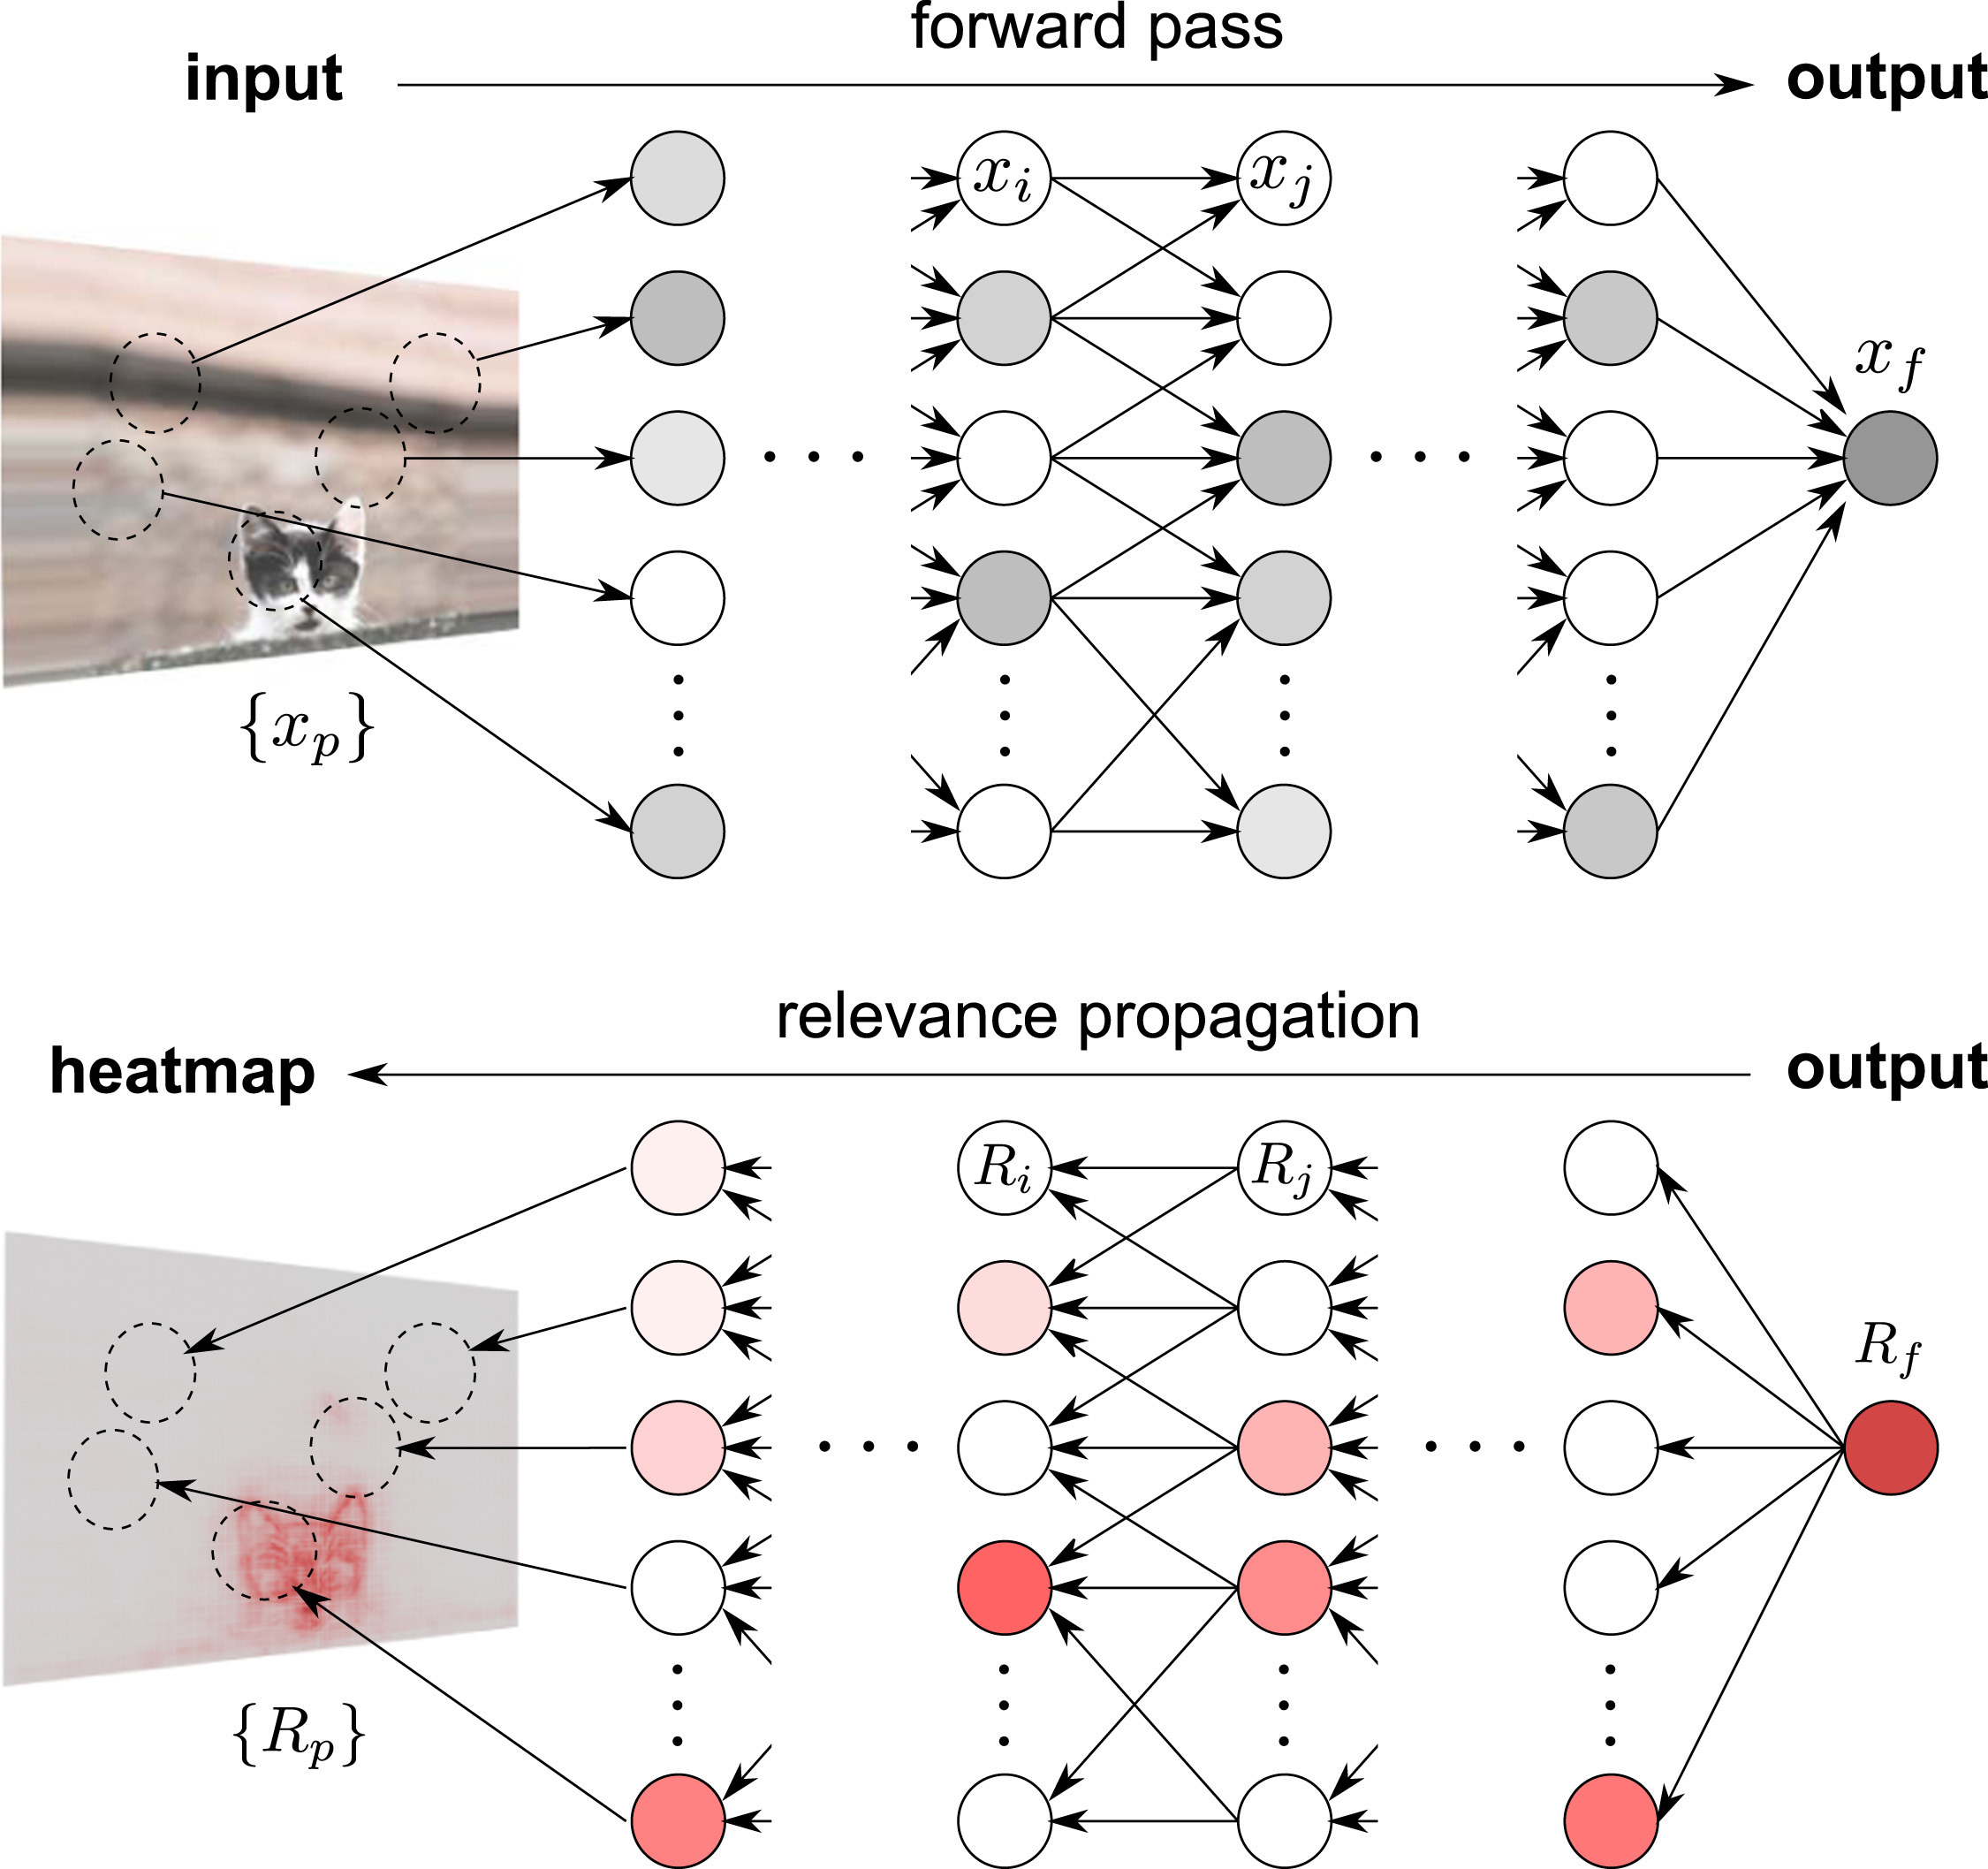
\includegraphics[width=\textwidth]{res/deep_taylor}
\end{center}
	\caption{Computational flow of deep Taylor decomposition. (Adopted from Montavon 2017).}
\end{figure}
\column{0.5\textwidth}
\begin{exampleblock}{}
The relevance in this framework can be defined as:
\begin{equation}
R_j = \sum _k \frac{a_j w_{jk}}{\sum _{0,j} a_j w_{jk}} R_k
\label{background:lrp.z}
\end{equation}
\end{exampleblock}
\end{columns}
\end{frame}



\section{Methods}

\subsection{Dataset}
%4.Material eksperymentalny

\begin{frame}
\frametitle{Dataset}
\begin{figure}
\begin{center}
  \includegraphics[width=0.7\textwidth]{res/dataset_structure}
\end{center}
	\caption{Speech corpus built originally for the purpose of the Polish BOSS unit selection synthesizer (Demenko, Bachan, M{\"o}bius 2008; Demenko, Klessa, Szyma\'nski, Breuer, Hess 2010).}
\end{figure}
\end{frame}

\begin{frame}
\frametitle{Dataset}
\begin{figure}
\begin{center}
  \includegraphics[width=0.4\textwidth]{res/dataset_structure_simple}
\end{center}
	\caption{Speech corpus built originally for the purpose of the Polish BOSS unit selection synthesizer (Demenko, Bachan, M{\"o}bius 2008; Demenko, Klessa, Szyma\'nski, Breuer, Hess 2010).}
\end{figure}
\end{frame}

\begin{frame}
\frametitle{Dataset}
\begin{center}
  \includegraphics[width=0.9\textwidth]{res/dataset_blf}
\end{center}
\end{frame}


\begin{frame}
\frametitle{Dataset}
\begin{center}
  \includegraphics[width=\textwidth]{res/database_structure_explanation}
\end{center}
\end{frame}

\subsection{Data preprocessing}

\begin{frame}
\frametitle{Data preprocessing}
\begin{center}
  \includegraphics[width=0.9\textwidth]{res/dataset_preprocessing}
\end{center}
\end{frame}


\subsection{Feature extraction}

\begin{frame}
\frametitle{Feature extraction}
\begin{center}
  \includegraphics[width=\textwidth]{res/dataset_feature_extraction}
\end{center}
\end{frame}

\subsection{Feature set}

\begin{frame}
\frametitle{Feature set}
\begin{columns}
\column{0.5\textwidth}
\begin{figure}
\begin{center}
  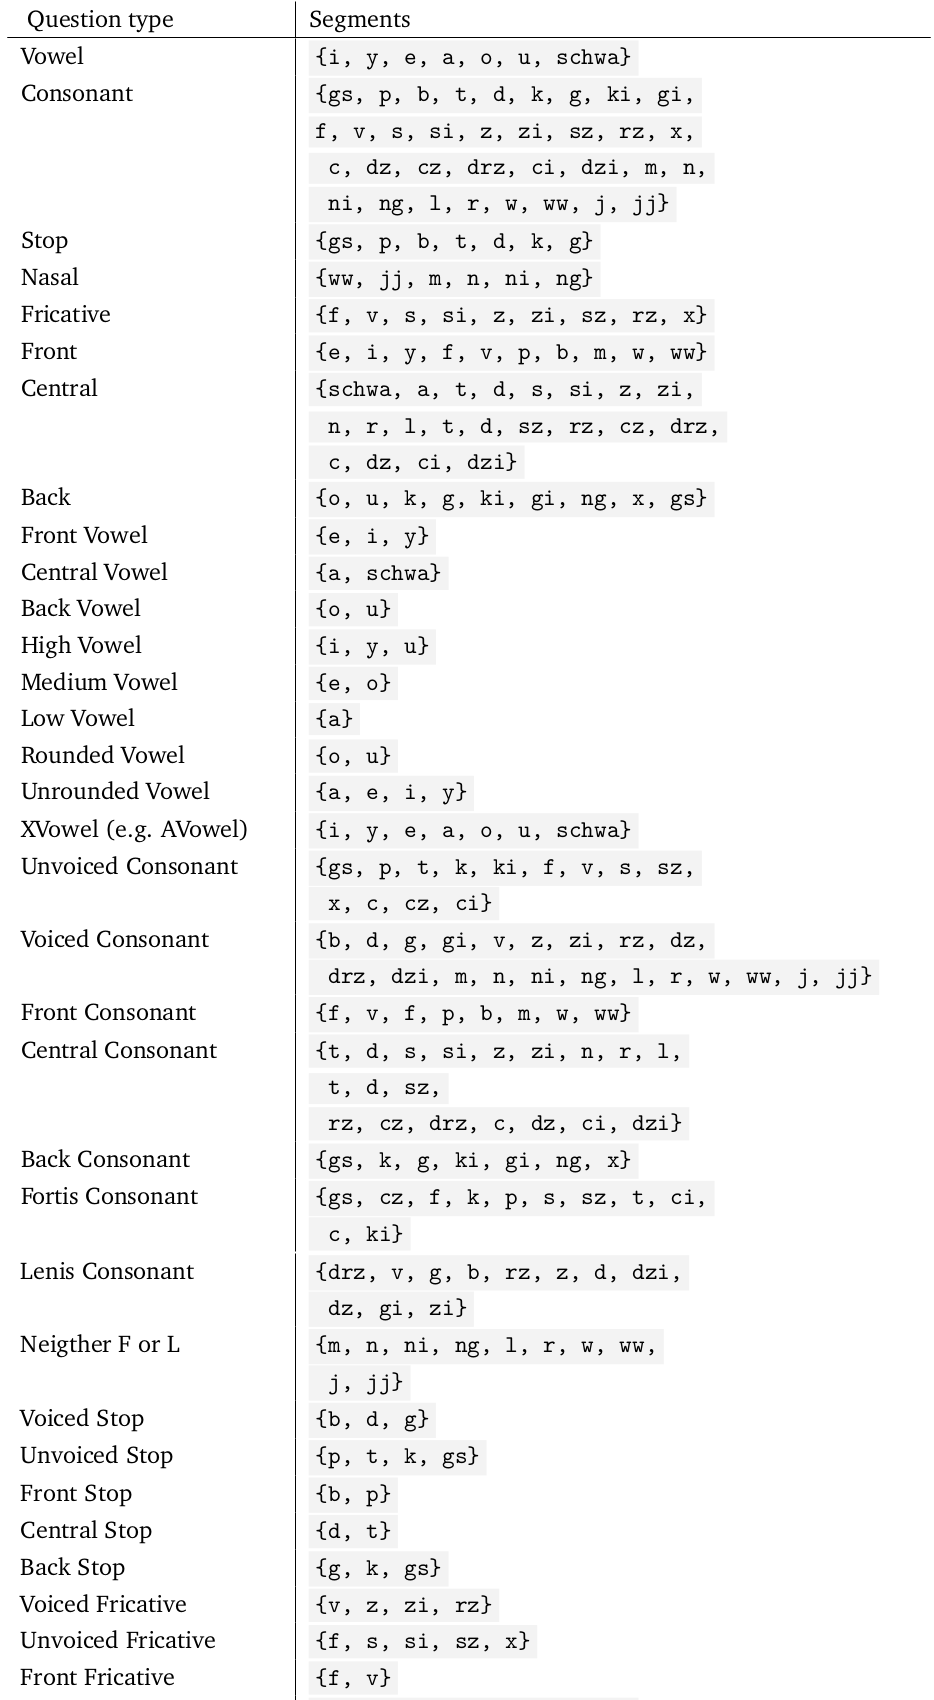
\includegraphics[width=0.6\textwidth]{res/segmental_features}
\end{center}
\caption{Segmental features for a quintphone-wide context.}
\end{figure}
\column{0.5\textwidth}
\begin{figure}
\begin{center}
  \includegraphics[width=0.8\textwidth]{res/suprasegmental_features}
\end{center}
\caption{Non-segmental features.}
\end{figure}
\end{columns}
\end{frame}

\subsection{Model implementation}

\begin{frame}
\frametitle{Model implementation}
\begin{columns}
\column{0.5\textwidth}
\begin{figure}
\begin{center}
  \includegraphics[width=0.6\textwidth]{res/residual_block}
\end{center}
\caption{Segmental features for a quintphone-wide context.}
\end{figure}
\column{0.5\textwidth}
\begin{center}
\includegraphics[width=2cm]{res/implementation_framework}
\end{center}
\hrule
\begin{exampleblock}{Complete code repository}
\begin{itemize}
\item[\checkmark] \scriptsize{\url{https://github.com/mrslacklines/intonation_synthesis}}
\end{itemize}
\end{exampleblock}
\end{columns}
\end{frame}


\section{Results}
%5. Wyniki

\subsection{Contribution}

\section{Hypotheses conclusions}
%6. Czy tezy zostaly udowodnione



\section{Future prospects}
%7. Aspekty przyszlosciowe i praktyczne

\begin{frame}

\begin{center}
Thank you.
\end{center}
\end{frame}










%%%%%%%%%%%%%%%%%%%%%%%%%%%%%%%%%%%%%%%%%%%%%%%%%%
% Additional slides
%%%%%%%%%%%%%%%%%%%%%%%%%%%%%%%%%%%%%%%%%%%%%%%%%%

\begin{frame}
\begin{figure}
\begin{center}
  \includegraphics[width=0.7\textwidth]{res/stress_accent_labels}
\end{center}
	\caption{Stress and accent labels used in the original Polish BOSS speech corpus.}
\end{figure}
\end{frame}

\begin{frame}
\begin{figure}
\begin{center}
  \includegraphics[width=0.7\textwidth]{res/boundary_tones}
\end{center}
	\caption{Prosodic phrase boundary labels used in the original Polish BOSS speech corpus.}
\end{figure}
\end{frame}

\begin{frame}
\begin{figure}
\begin{center}
  \includegraphics[width=0.4\textwidth]{res/tonal_accents}
\end{center}
	\caption{Acoustic realizations of the 9 different accents. Adopted from (Demenko 1999).}
\end{figure}
\end{frame}


\end{document}
